\documentclass{article}
\usepackage[utf8]{inputenc}
\usepackage{amsmath}
\usepackage{graphicx}

% Better line breaks between paragraphs and no indentes
\usepackage[parfill]{parskip}

% To get better spacing with itemized lists
\usepackage{enumitem}
\setlist{nosep,after=\vspace{\baselineskip}}

% For creating augmented matricies
\newenvironment{amatrix}[1]{%
    \left[\begin{array}{@{}*{#1}{c}|c@{}}
} {%
    \end{array}\right]
}

% Creating math equation tags
\newcommand\addtag{\refstepcounter{equation}\tag{\theequation}}

\title{CSYS 300 PoCS Assignment 4}
\author{Thomas Waters}
\date{September 28th 2018}

\begin{document}

\maketitle
Code is located at

https://github.com/Evelios/PoCS\_Assignment\_04

%--------------------------------------------------------------
\section{Problem 1}
Adding some content to problem 1

\section{Problem 2}
Normalized number of groups inthe long time limit, $n_k$ satisfies the following difference equation with $k \geq 2$,

\[
  \frac{
    n_k
  }{
    n_{k-1}
  }
  =
  \frac{
    (k - 1)(1 - \rho)
  }{
    1 + (1 - \rho)k
  }
  \addtag
\]

For $k=1$,

\[
  n_1
  =
  \rho - (1 - \rho) n_1
  \addtag
\]

The following steps are to derive the exact solution for $n_k$. The following derivation will use both the gamma function and the beta function with the following definitions,

\[
  \Gamma(x) = (k - 1)!
  \addtag
\]

\[
  \beta(x, y) =
  \frac{
    \Gamma(x) \Gamma(y)
  }{
    \Gamma(x + y)
  }
  \addtag
\]

So now simplifying for $n_k$

\[
  \frac{
    n_k
  }{
    n_{k-1}
  }
  =
  \frac{
    (k - 1)(1 - \rho)
  }{
    1 + (1 - \rho)k
  }
  \addtag
\]

% Starting Recursion

\[
  n_k
  =
  \frac{
    (k - 1)(1 - \rho)
  }{
    1 + (1 - \rho)k
  }
  n_{k-1}
  \addtag
\]

\[
  =
  \left[
    \frac{
      (k - 1)(1 - \rho)
    }{
      1 + (1 - \rho)k
    }
  \right]
  \left[
    \frac{
      (k - 2)(1 - \rho)
    }{
      1 + (1 - \rho)(k - 2)
    }
  \right]
  n_{k-2}
  \addtag
\]

\[
  =
  \left[
    \frac{
      (k - 1)(1 - \rho)
    }{
      1 + (1 - \rho)k
    }
  \right]
  \left[
    \frac{
      (k - 2)(1 - \rho)
    }{
      1 + (1 - \rho)(k - 2)
    }
  \right]
  ...
  n_2
  n_1
  \addtag
\]

\[
  =
  \left[
    \frac{
      (k - 1)(1 - \rho)
    }{
      1 + (1 - \rho)k
    }
  \right]
  \left[
    \frac{
      (k - 2)(1 - \rho)
    }{
      1 + (1 - \rho)(k - 1)
    }
  \right]
  ...
  \left[
    \frac{
      (2 - 1)(1 - \rho)
    }{
      1 + (1 - \rho)(2)
    }
  \right]
  n_1
  \addtag
\]

% Solving for the gamma function

\[
  =
  \frac{
    (1 - \rho)^{k - 1}
  }{
    (1 - \rho)^{k - 1}
  }
  \left[
    \frac{
      (k - 1)
    }{
      \frac{1}{1 - \rho} + k
    }
  \right]
  \left[
    \frac{
      (k - 2)
    }{
      \frac{1}{1 - \rho} + (k - 1)
    }
  \right]
  ...
  \left[
    \frac{
      (2 - 1)
    }{
      \frac{1}{1 - \rho} + (2)
    }
  \right]
  n_1
  \addtag
\]

\[
  =
  \Gamma(k)
  \left[
    \frac{
      1
    }{
      \frac{1}{1 - \rho} + k
    }
  \right]
  \left[
    \frac{
      1
    }{
      \frac{1}{1 - \rho} + (k - 1)
    }
  \right]
  ...
  \left[
    \frac{
      1
    }{
      \frac{1}{1 - \rho} + (2)
    }
  \right]
  n_1
  \addtag
\]

\[
  n_k
  =
  \frac{
    \Gamma
    \left(
      k
    \right)
    \Gamma
    \left(
      1 - \rho + 1
    \right)
  }{
    \Gamma
    \left(
      1 - \rho + 1 + k
    \right)
  }
  n_1
  \addtag
\]

\[
  n_k
  =
  \frac{
    \Gamma
    \left(
      k
    \right)
    \Gamma
    \left(
      \rho
    \right)
  }{
    \Gamma
    \left(
      \rho + k
    \right)
  }
  n_1
  \addtag
\]

% Applying the beta function

\[
  n_k
  = 
  \beta
  \left(
    k,
    \rho
  \right)
  n_1
  \addtag
\]

\section{Problem 3}
From the lectures we arrived at the following,

\[
  \gamma
  =
  1 + 
  \frac{1}{
    1 - \rho
  }
  \addtag
\]

For $\rho \to 0$,
\[
  \gamma
  =
  \lim_{\rho \to 0}
  1 + 
  \frac{1}{
    1 - \rho
  }
  =
  2
  \addtag
\]

For $\rho \to 1$,
\[
  \gamma
  =
  \lim_{\rho \to 1}
  1 + 
  \frac{1}{
    1 - \rho
  }
  =
  \infty
  \addtag
\]

For the case of $\gamma \to 2$, there is no mutation rate and the entire population is in the same grounp, this would cause the slope of the distribution to become infinite because there would be nothing to scale against. In the case where $\gamma \to \infty$, we are guarenteed to make a new group every time. This would cause the frequency of all the groups to be one, causing the power law slope to go to zero because each group occurs as often as every other one.

\section{Problem 4}
\[
  n_1
  =
  \frac{
    \rho
  }{
    2 - \rho
  }
  \addtag
\]

\[
  n_k^{(g)}
  =
  \frac{1}{\rho t}
  N_{k t}
  =
  \frac{1}{\rho}
  n_k
  \addtag
\]

Solving for $n_2^{(g)}$,

\[
  \frac{
    n_k
  }{
    n_{k-1}
  }
  =
  \frac{
    (k - 1)(1 - \rho)
  }{
    1 + (1 - \rho)k
  }
  \addtag
\]

\[
  n_k
  =
  \frac{
    (k - 1)(1 - \rho)
  }{
    1 + (1 - \rho)k
  }
  n_{k-1}
  \addtag
\]

\[
  n_2
  =
  \frac{
    (2 - 1)(1 - \rho)
  }{
    1 + (1 - \rho)2
  }
  n_1
  \addtag
\]

\[
  n_2
  =
  \frac{
    (1 - \rho)
  }{
    1 + 2(1 - \rho)
  }
  \left[
    \frac{
      \rho
    }{
      2 - \rho
    }
    \right]
  \addtag
\]

\[
  n_2^{(g)}
  =
  \frac{1}{\rho}
  n_2
  =
  \frac{1}{\rho}
  \left[
    \frac{
      1 - \rho
    }{
      3 - 2\rho
    }
  \right]
  \left[
    \frac{
      \rho
    }{
      2 - \rho
    }
  \right]
  \addtag
\]

\[
  n_2^{(g)}
  =
  \frac{
    (1 - \rho)
  }{
    (2 - \rho)
    (3 - 2\rho)
  }
  \addtag
\]

Now for $n_3^{(g)}$,

\[
  n_k
  =
  \frac{
    (k - 1)(1 - \rho)
  }{
    1 + (1 - \rho)k
  }
  n_{k-1}
  \addtag
\]

\[
  n_3
  =
  \frac{
    (3 - 1)(1 - \rho)
  }{
    1 + (1 - \rho)3
  }
  n_{2}
  \addtag
\]

\[
  n_3
  =
  \frac{
    2(1 - \rho)
  }{
    4 - 3\rho
  }
  \left[
    \frac{
    (1 - \rho)
  }{
    3 - 2\rho
  }
  \right]
  \left[
    \frac{
      \rho
    }{
      2 - \rho
    }
  \right]
  \addtag
\]

\[
  n_3^{(g)}
  =
  \frac{1}{\rho t}
  N_{3 t}
  =
  \frac{1}{\rho}
  n_3
  \addtag
\]

\[
  n_3^{(g)}
  =
  \frac{1}{\rho}
  \left[
    \frac{
      2(1 - \rho)
    }{
      4 - 3\rho
    }
  \right]
  \left[
    \frac{
    (1 - \rho)
  }{
    3 - 2\rho
  }
  \right]
  \left[
    \frac{
      \rho
    }{
      2 - \rho
    }
  \right]
  \addtag
\]

\[
  n_3^{(g)}
  =
  \frac{
    2 (1 - \rho)^2
  }{
    (4 - 3\rho)
    (3 - 2\rho)
    (2 - \rho)
  }
\]

\section{Problem 5}
Here I am using the Hurwitz Zeta Function,
\[
  \zeta
  \left(
    s, q
  \right)
  =
  \sum_{n = 0}^{\infty}
  \frac{1}{(q + n)^s}
\]

Trying to estimate the minimum of the largest sample in the network.

\[
  P_k =
  c k^{-\gamma}
  \addtag
\]

\[
  \sum_{k = min \, k_{max}}^{\infty}
  P_k
  =
  \frac{1}{N}
  \addtag
\]

\[
  \sum_{k = min \, k_{max}}^{\infty}
  c k^{-\gamma}
  =
  \frac{1}{N}
  \addtag
\]

\[
  c
  \sum_{k = min \, k_{max}}^{\infty}
  \frac{1}{k^{\gamma}}
  =
  \frac{1}{N}
  \addtag
\]

\[
  c
  \sum_{k = 0}^{\infty}
  \frac{1}{
    \left(
      (min \, k_{max}) + k
    \right)^{\gamma}
  }
  =
  \frac{1}{N}
  \addtag
\]

\[
  c \,
  \zeta
  \left(
    \gamma, min \, k_{max}
  \right)
  =
  \frac{1}{N}
  \addtag
\]

\section{Problem 6}
Unfortunately on this one, the plots out of R on such small scales caused some problems for both the titles and the labels.

Showing $k_max$ for $N = 10^1$ (left) and for $N = 10^2$ (right).

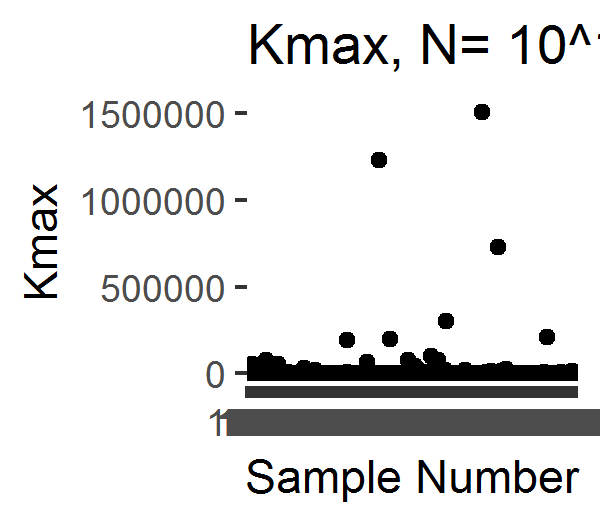
\includegraphics{../images/Problem6_10^1.png}
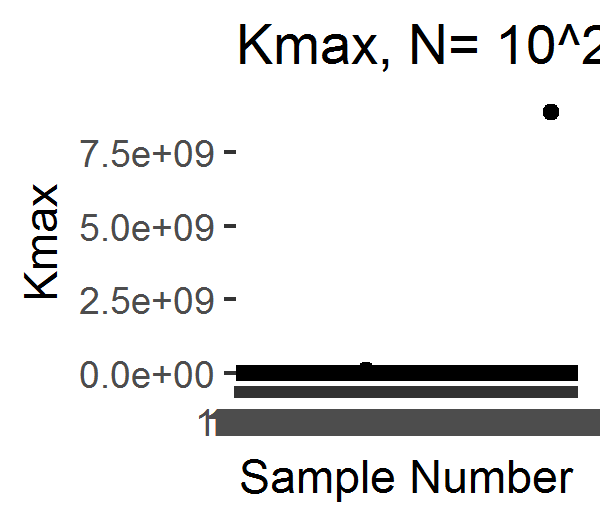
\includegraphics{../images/Problem6_10^2.png}

Showing $k_max$ for $N = 10^3$ (left) and for $N = 10^4$ (right).

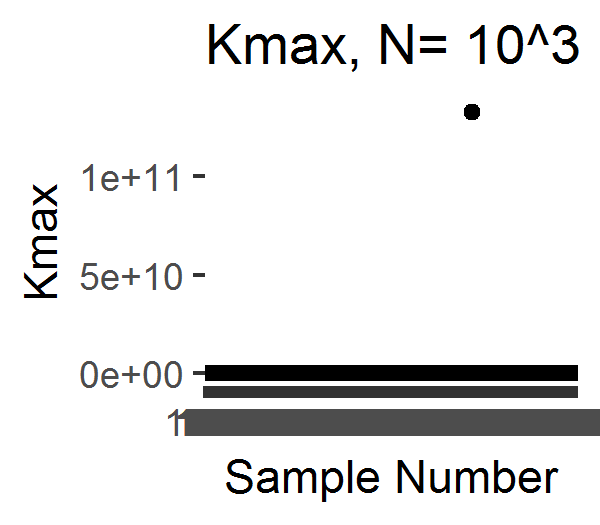
\includegraphics{../images/Problem6_10^3.png}
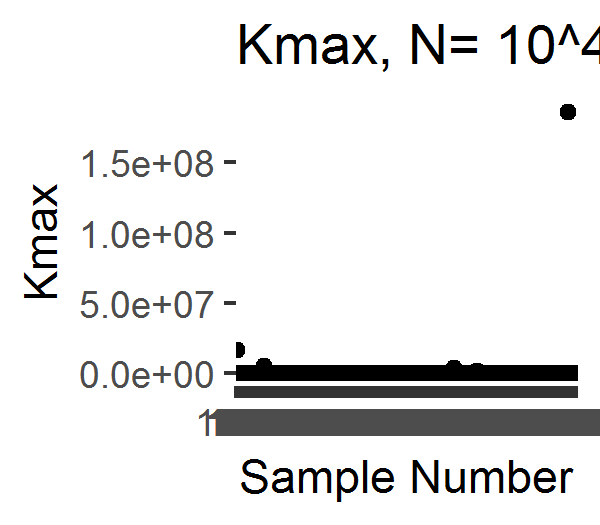
\includegraphics{../images/Problem6_10^4.png}

Showing $k_max$ for $N = 10^5$ (left) and for $N = 10^6$ (right).

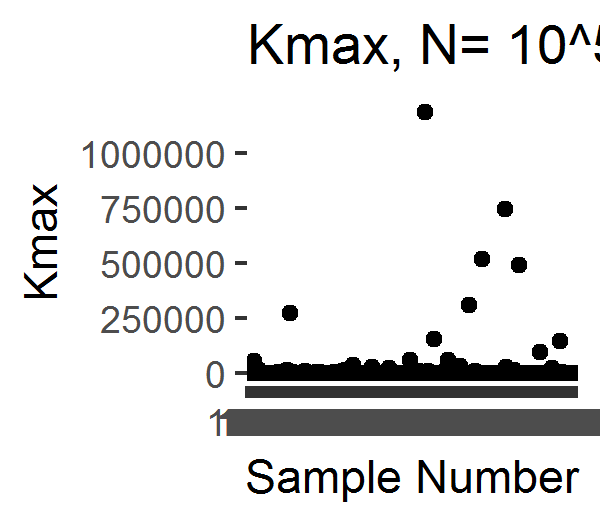
\includegraphics{../images/Problem6_10^5.png}
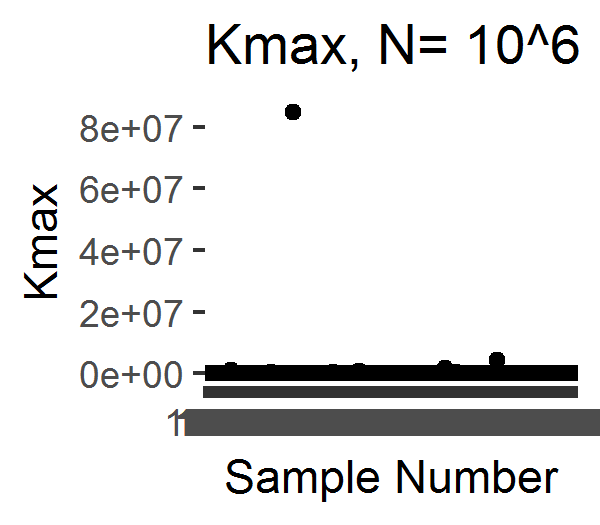
\includegraphics{../images/Problem6_10^6.png}

Unfortunately for this homework it seems that again, something is off. Here, unfortunately because of the nature of power law distributions I can't tell if it is the nature of the distribution but I assume it is probably a result of my algorithm. Here, I would expect from the averaging from 1000 simulation that any of the erratic behavior from the output of the power law distributions would be mitigated. Here, unfortunately, from my graph of the average for $k_max$, I don't see any relationship in the average value of $k_max$ in terms of the sample size.

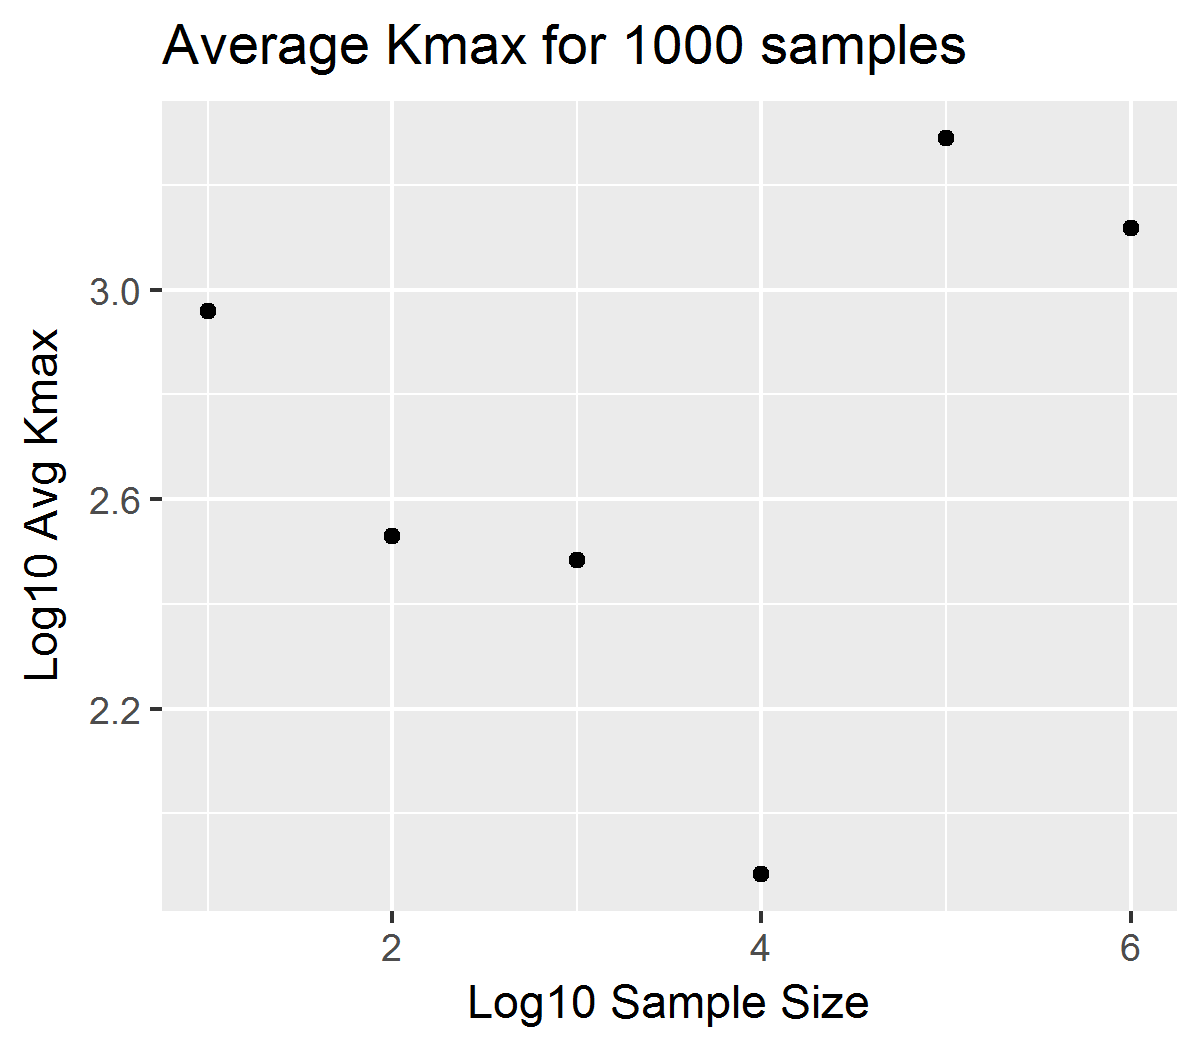
\includegraphics{../images/Problem6_average_max.png}

\section{Problem 7}
Using a 1D random walk. If the walker starts at $x = i$, I will show how many distinct random walks there are that reach $x = j$ after $t$ time steps. Let $P$ be the number of positive steps taken and $N$ be the number of negative steps taken.

Because the walker must take $t$ steps and they must be either positive or negative,
\[
    P + N = t
    \addtag
\]

I am also only looking at the number of steps that reach $(j - i)$ (the distance traveled) steps away,
\[
    P - N = j - i 
    \addtag
\]

The number of possible random walks is also given by $N(i, j, t)$ is,
\[
    N(i, j, t) = 
        \binom{t}{P}
    \addtag
\]

Simplifying the equations starting with (2) and then substituting into (1) and then (3).
\begin{equation}
\begin{gathered}
    P - N = j - i
    P  = j - i + N
    P - j + i = N
\end{gathered}
\end{equation}

\[
    N = P - j + i
    \addtag
\]

Substituting (5) into the equation from (1)
\begin{equation}
\begin{gathered}
    P + N = t
    P + (P - j + i) = t
    2P - j + i = t
    2P = t + j - i
\end{gathered}
\end{equation}

\[
    P = (t + j - i) / 2
    \addtag
\]

\begin{equation}
\begin{gathered}
    N(i, j, t) =
        \binom{t}{P} \\
    N(i, j, t) =
        \binom{t}{(t + j - i) / 2}
\end{gathered}
\end{equation}

\section{Problem 8}
\input{problem8.tex}

\end{document}

